\chapter{Result \& Discussion}
\section{Powder characteristics}
\subsection{Size distribution}
According to previous research, the nanoparticles with a size of tens of nanometers are defined as primary particles,  the particles with the size of 0.1 to 1 $\mathrm{\mu m}$ are defined as secondary particle, and likewise, those particles with larger sizes are defined as tertiary and quaternary particles.
As Fig. 4。1 shows, it is confirmed that the pure Si nanoparticles exhibit a large bump from 0.1 to 10 µm and major of them are within 1 to 10 $\mathrm{\mu m}$. The size distribution of pure Si nanoparticles  is uniform. On the other hand, with Ni addition, there are two major peaks with the center around 0.1 $\mathrm{\mu m}$ and 10~20 $\mathrm{\mu m}$, which indicates that the Ni addition induce partly agglomeration of nanoparticles. 
\begin{figure}[H]
\centering
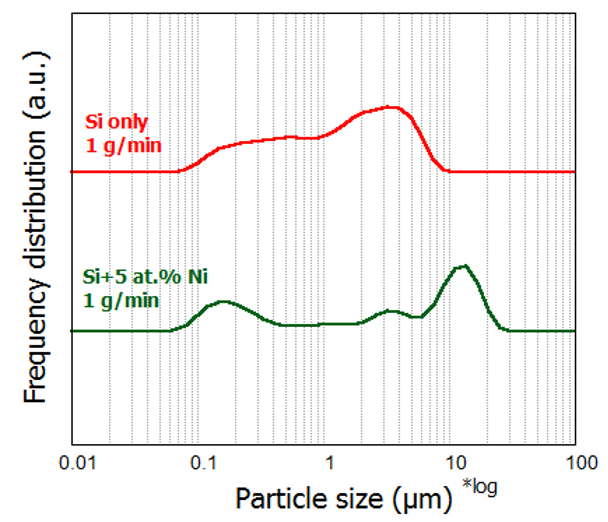
\includegraphics[width=8cm]{src/fig/fig42.png}
\caption{Particle size distribution.}
\end{figure}
\newpage
\subsection{Particle morphology}
The surface morphologies of the PS-PVD processed Si nanocomposites with and without Ni addition  is revealed by SEM. As figure 4.2 shows,  the raw mg-Si powder is about 20 µm on average and in a sharp-cornered shape. In contrast, the size of PS-PVD processed nanoparticles are significantly reduced and exhibits a more spherical shape. Due to limited amount of Ni addition, the morphology of processed Si:Ni nanoparticles are similar to that of Si-only nanoparticles, samely reduced size and spherical shape. That is, the 5 at.\% Ni addition can not make significantly change to nanoparticle morphology.
\begin{figure}[h]
\centering
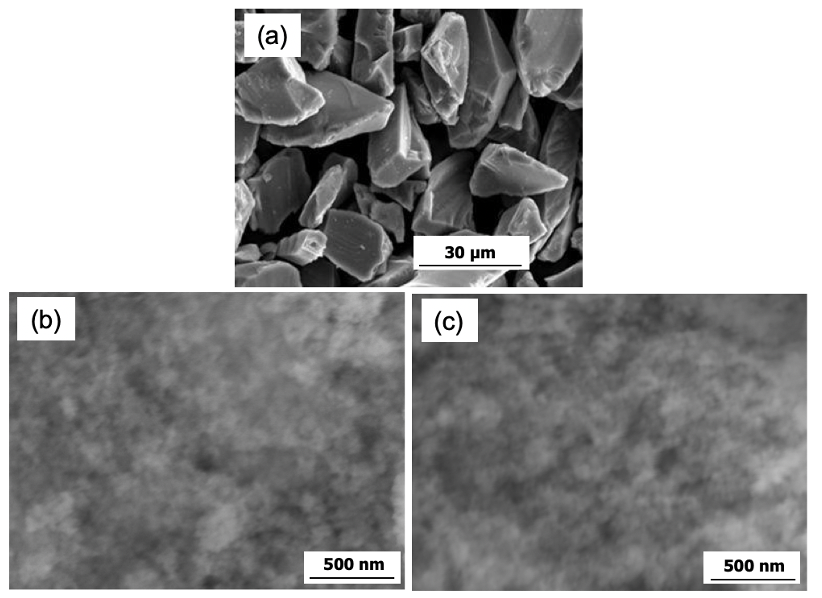
\includegraphics[width=12cm]{src/fig/fig43.png}
\caption{SEM micrograpghs of  PS-PVD processed powders (a) raw powder(MG-Si); (b) Si-only particles; (c) Si:Ni particles}
\end{figure}
\begin{figure}[h]
\centering
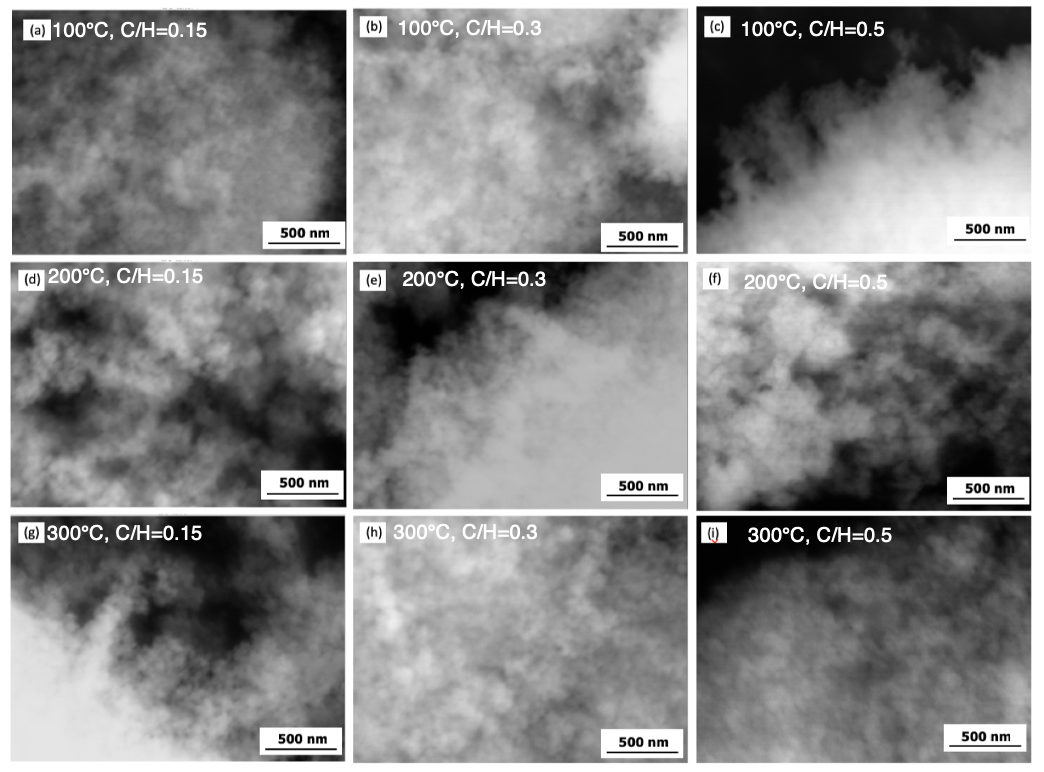
\includegraphics[width=12cm]{src/fig/fig44.png}
\caption{SEM images of PE-CVD post annealed nanopowders at different temperature and gas ratios}
\end{figure}

Figure 4.3 shows the SEM micrograpghs of the PE-PVD post annealed Si:Ni nanoparticles at different temperature and gas ratios. It’s clear that the post-annealing has not significantly change the morphology of nanoparticles. Unfortunately, the rod-like materials is not found. 

The possible reasons might be: 
\begin{itemize}
  \item Carbon nanotubes do grow, but are to short or hidden in this cotton-like nanostructure to be distinguished due to limited resolution of SEM.
  \item Carbon nanotubes is not grown, instead, carbon deposited on Si:Ni-NPs in the form of amorphous carbon, which is inferred by EDS analysis. 
\end{itemize}
\newpage
Figure 4.4 the EDS mapping illustrates the distribution of elements in PE-CVD post annealed powders. It’s clear that the major element is Si, and other elements like Ni, C and O are uniformly distributed on Si nanoparticles. The EDS energy spectrum also reveal the presence of carbon in a qualitative way. The presence of Oxygen feature is probably due to an exposure of the samples to air.
\begin{figure}[H]
\centering
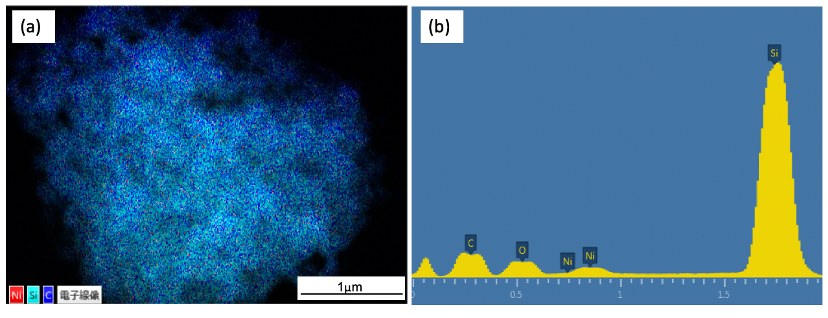
\includegraphics[width=12cm]{src/fig/fig45.png}
\caption{(a) Si, C, Ni, and O element mapping by EDS. (b)element content.}
\end{figure}
\newpage
%拉曼
\subsection{Raman spectroscopy}
Figure 4.6 shows the Raman spectroscopy of 200\(^\circ\)C annealed powder with different gas ratio. In the range of 200 to 1800 $\mathrm{cm^{-1}}$, only the peak responsible for crystalline Si exist(500\(^\circ\)). Especially around 1380 $\mathrm{cm^{-1}}$ (D peak) and 1600 $\mathrm{cm^{-1}}$(G peak), the intensity is close to zero. It implies that the carbon nanotubes is not successfully grown.  
\begin{figure}[h]
\centering
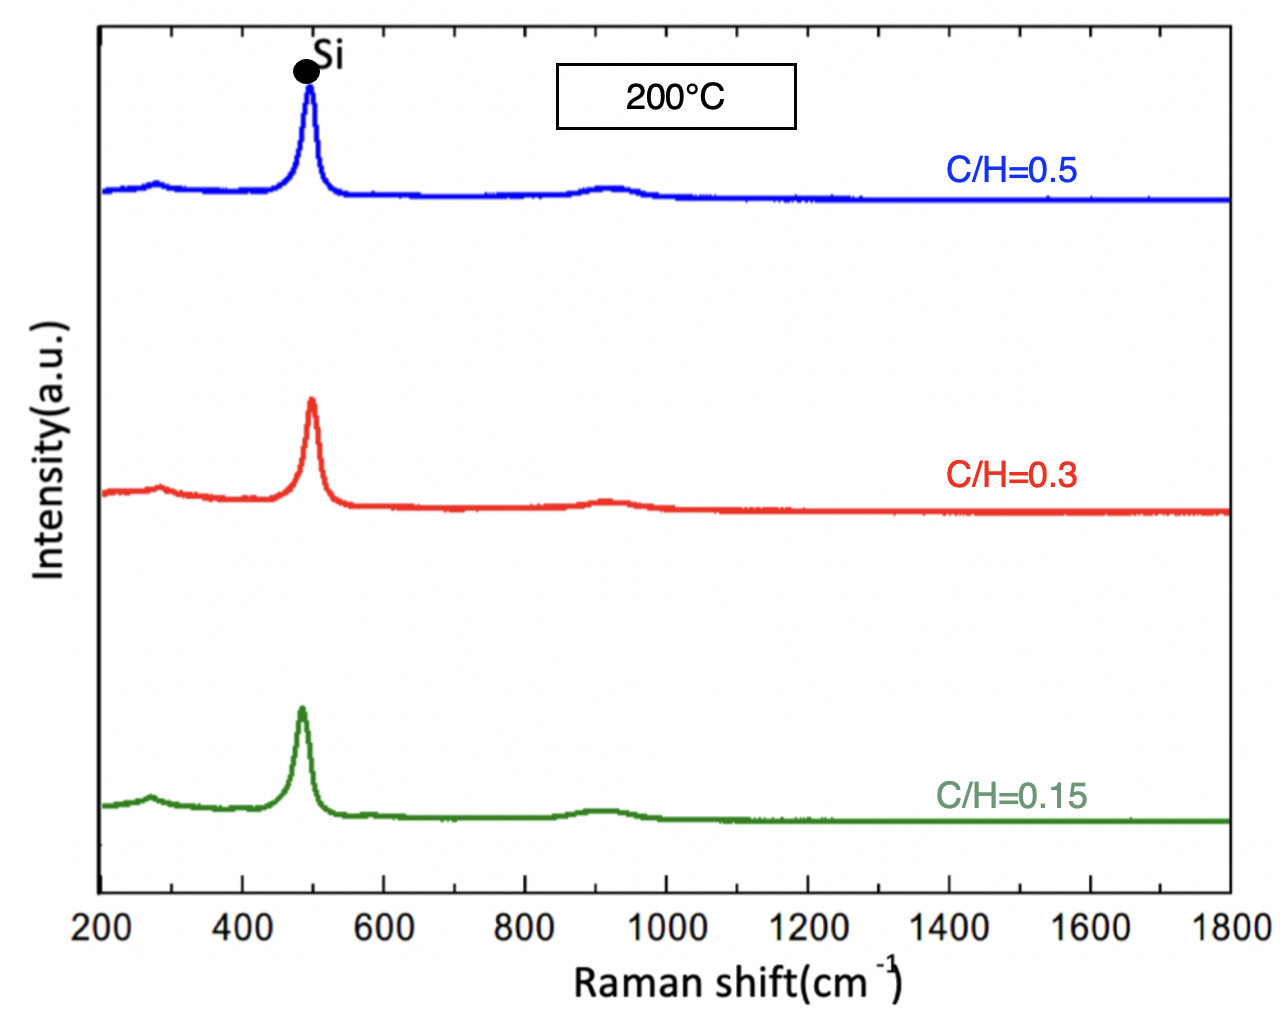
\includegraphics[width=8cm]{src/fig/fig46.png}
\caption{Raman spectroscopy of annealed Si:Ni powders at 200\(^\circ\)C}
\end{figure}
%XRD
\subsection{Phase analysis}
\begin{figure}[h]
\centering
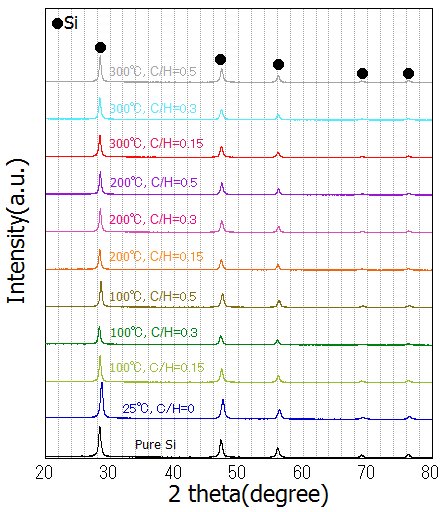
\includegraphics[width=8cm]{src/fig/fig47.png}
\caption{XRD pattern of powders}
\end{figure}
The deference in XRD patterns of annealed powders at different temperature and gas ratio is indistinct. Due to small amount of Ni addition and relatively low temperature annealing, even $\mathrm{Ni_{x}Si}$ phase exist. It’s difficult to distinguish with comparison to the towering Si peak.
\begin{table}[H]
\caption{Rietveld analysis of silicidation at different temperature}
\begin{tabular}{ccccccc}
\toprule
\begin{array}{c}
\text {Temperature} \\
\text {(\(^\circ\)C)}
\end{array}  &  
\begin{array}{c}
\text {Si } \\
\text {(at.\%)}
\end{array}&
\begin{array}{c}
\text {$\mathrm{NiSi_{2}}$} \\
\text {(at.\%)}
\end{array}    & 
\begin{array}{c}
\text {$\mathrm{NiSi}$} \\
\text {(at.\%)}
\end{array}    &  
\begin{array}{c}
\text {$\mathrm{Ni_{2}Si}$} \\
\text {(at.\%)}
\end{array}    & 
\begin{array}{c}
\text {Ni} \\
\text {(at.\%)}
\end{array}  & \begin{array}{c}
\text {Ni Remained} \\
\text {(at.\%)}
\end{array} 
\\ \midrule
25 & 96.45 & 0.90 & 0.70 & 0.88 & 1.06 & 100.00       \\
10& 96.02 & 1.49 & 0.99 & 0.61 & 0.90 & 84.56     \\
200 & 96.13 & 1.35 & 1.12 & 0.72 & 0.68 & 64.26     \\
300 & 94.68 & 2.17 & 1.73 & 1.20 & 0.26 & 24.56     \\ \bottomrule
\end{tabular}
\end{table}
The degree of  Ni silicidation is quantified in the way of considering the relative amount of pure Ni before and after annealing. It’s believed that the gas ratio is of little effect to Ni silicidation, so the Rietveld analysis result is carried out among powders with fixed gas ratio(C/H=0.15). Dividing the amount of Ni after annealing by that of Ni before annealing(RT), the percentage of unconsumed Ni amount is obtained. Compare this result to simulation, for 100\(^\circ\)C case, the simulation suggests no silicidation occurs. But from Rietveld analysis result, silicidation consumes about 15 at.\% of Ni. Additionally, at 200\(^\circ\)C, the simulation shows $\sim$ 75 at.\% is remain unconsumed and Rietveld analysis shows 84.56 at.\%. At 300\(^\circ\)C, the simulation shows it’s limit that it’s not applicable to  higher temperature. But the Rietveld analysis demonstrate the relatively serious Ni silicidation for about 80 at.\% Ni atoms are involved in.
\begin{figure}[H]
\centering
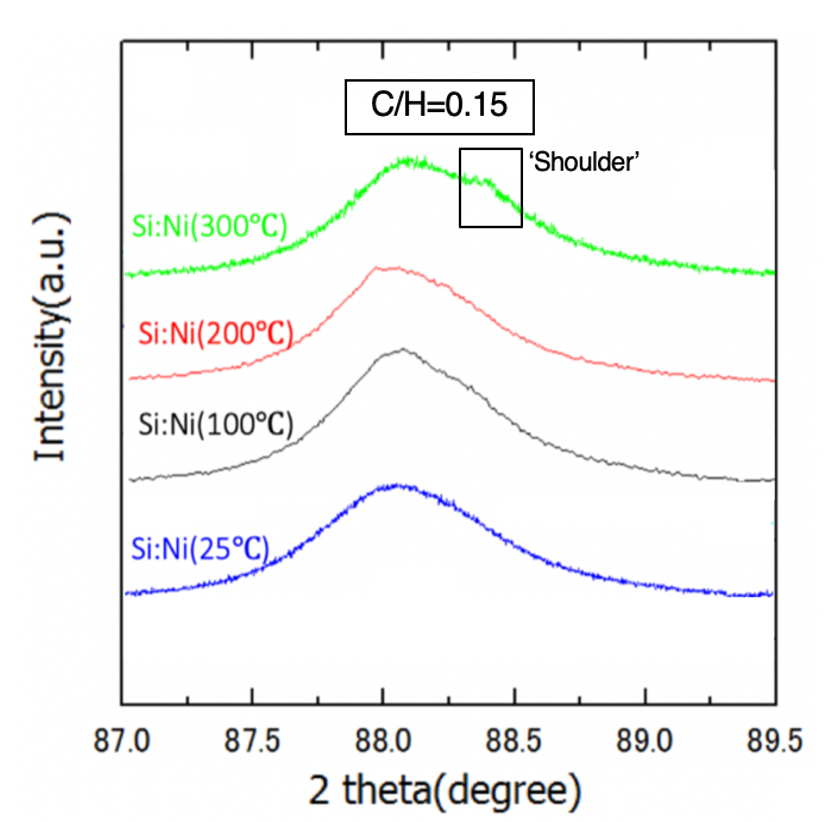
\includegraphics[width=8cm]{src/fig/fig48.png}
\caption{High angle(87$\sim$90\(^\circ\)) XRD pattern of powders at different temperature with a fixed gas ratio of C/H=0.15}
\end{figure}
From figure 4.7, it’s clear that the high angle XRD pattern of 25\(^\circ\)C, 100\(^\circ\)C, 300℃\(^\circ\)C are similarly shaped. But the 300\(^\circ\)C powders exhibit a shoulder around 88.4\(^\circ\). Thus peak fitting was performed using Origin Pro in Origin Lab. The two theta values used for distinguish silicide peaks are:
$$ \mathrm{Si}: 88.029^{\circ} \qquad  \mathrm{NiSi_{2}}: 88.390^{\circ}\qquad  \mathrm{Ni_{2}Si}: 88.673^{\circ}\qquad \mathrm{ NiSi}: 88.796^{\circ}$$
\begin{figure}[H]
\centering
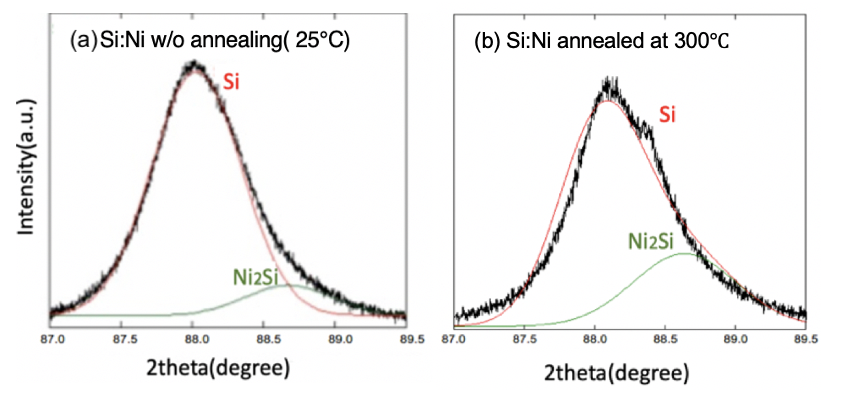
\includegraphics[width=12cm]{src/fig/fig49.png}
\caption{peak fitting of Si:Ni particles (a)without annealing  and (b)  annealed at 300\(^\circ\)C }
\end{figure}
The peak fitting result shown in figure 4.8 indicates an increase of $\mathrm{NiSi_{2}}$ phase content after annealing at 300\(^\circ\)C, further confirms that such right-shifted shoulder is due to Ni silicide. \\
\subsection{Si carbonous structure by TEM}
\begin{figure}[H]
\centering
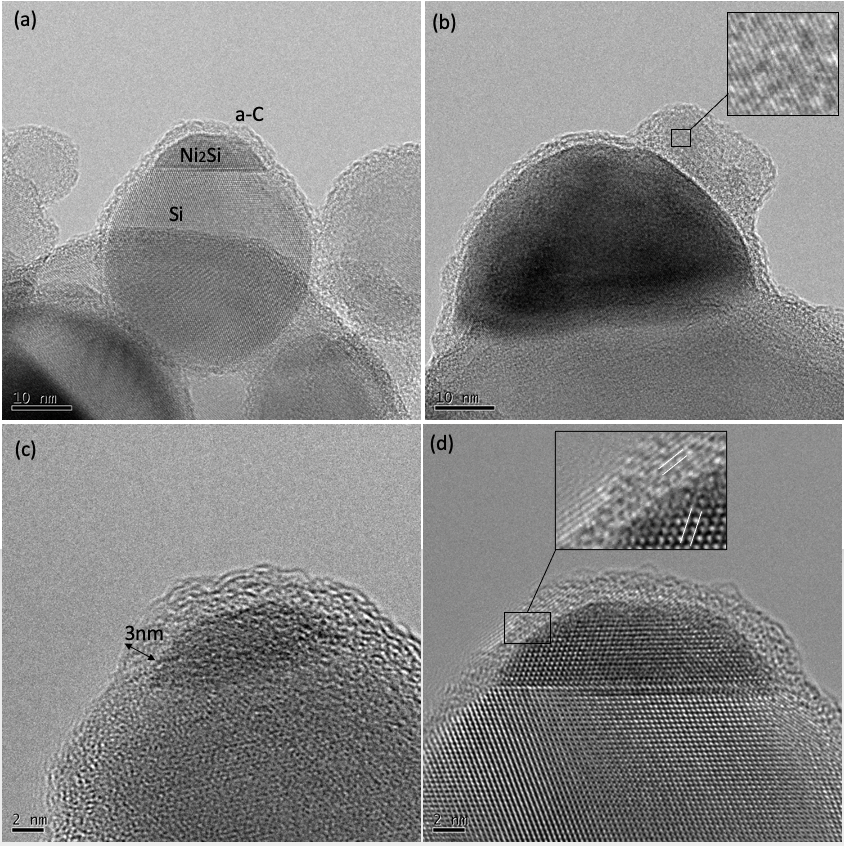
\includegraphics[width=8cm]{src/fig/fig50.png}
\caption{FE-TEM image of Si:Ni:C nanoparticle}
\end{figure}
The TEM image further confirms the nanostructure in which Ni cap is directly attached on the Si nanoparticle. The diameter of Si is 20$\sim$30 nm and the size of radius of Ni is $\sim$10 nm. From figure 4.9, it’s seen that the particle is encapsulated in an amorphous coating with a uniform thickness of $\sim$3 nm. Figure. 4.9(b) and (d) shows the existence of crystalline part in amorphous carbon coating. Especially in (b), the rod extruded from Ni surface is inferred to be the nuclei of CNT.  From figure (c), it’s clear that the Ni silicidation takes place and almost the entire Ni transformed into $\mathrm{Ni_{2}Si}$ phase. 
  
Since it’s confirmed by TEM observation that amorphous carbon coating forms on Si:Ni:C-NP surface instead of CNT. Still, we can use the same mathematics model to calculate the thickness of amorphous carbon coating.  The length of CNT at different growth condition is obtained by simulation. With known the areal density of carbon and the carbon atomic radius, the convert the CNT length into thickness. 
\begin{center}
    &\text { Table. } 4.2 \text { Length of CNT and thickness of a-C coating }
\end{center}
$$
\begin{aligned}
&\begin{array}{|c|c|c|c|c|c|c|c|c|c|}
\hline \text { Temperature }\left({ }^{\circ} \mathrm{C}\right) & \multicolumn{3}{|c|} {100} & \multicolumn{3}{|c|} {200} & \multicolumn{3}{|c|} {300} \\
\hline \text { C/H } & 0.15 & 0.3 & 0.5 & 0.15 & 0.3 & 0.5 & 0.15 & 0.3 & 0.5 \\
\hline \begin{array}{c}
\text { Length } \\
\text { of CNT (nm) }
\end{array} & 37.8 & 47.98 & 57.19 & 161.5 & 208.09 & 250 & 410 & 535.5 & 655 \\
\hline \begin{array}{c}
\text { Thickness } \\
\text { of a-C coating(nm) }
\end{array} & 0.6 & 0.761 & 0.907 & 2.56 & 3.3 & 3.98 & 6.5 & 8.49 & 10.4 \\
\hline
\end{array}
\end{aligned}
$$
 The thickness  of a-C coating observed by TEM is 3 nm and according to simulation it should be 10.4 nm. The possible reason accounts for this phenomenon are as follows. First, the mathematics model assume flowing $\mathrm{C_{2}H_{2}}$ is totally decomposed, which in general difficult. Second,   the NH3  etching effect is ignored. So simulation usually get a larger value of product. It’s reasonable that the actual thickness is smaller than simulated thickness.
 \newpage
 \section{Battery performance}
 It's known that amorphous carbon coating can improve the specific capacity of Si nanoparticles due to its flexibility and enhance electrical conductivity. As for the Ni silicide formed during annealing, since it consumes part of Si, it reduces the theoretical capacity. 
・reduce resistance
\begin{figure}[H]
\centering
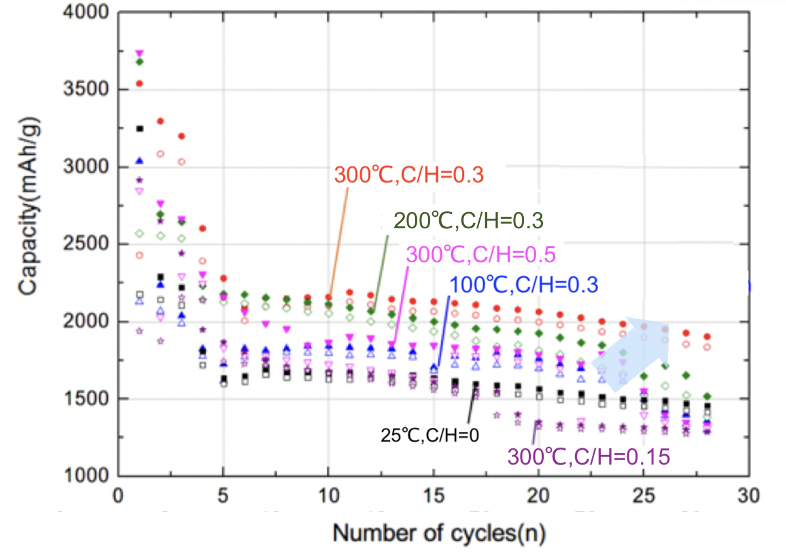
\includegraphics[width=8cm]{src/fig/fig51.png}
\caption{The specific capacity of annealed Si:Ni:C-NP in 30 cycles}
\end{figure}
\begin{figure}[H]
\centering
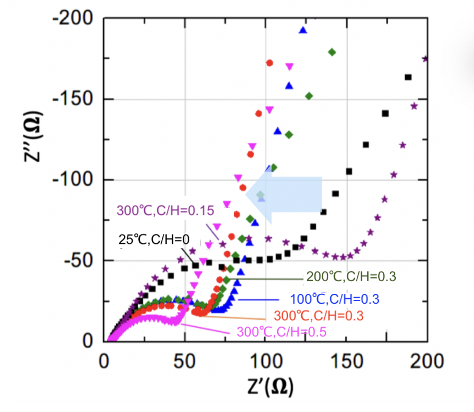
\includegraphics[width=8cm]{src/fig/fig52.png}
\caption{The impedance of annealed Si:Ni:C-NPs}
\end{figure}

\subsubsection{C/H dependence}
\noindent $\bullet$ Specific capacity\\
According to figure 4.10, at 300\(^\circ\)C the specific capacity sequence is: 
$$\mathrm{[C/H=0.3] > [C/H=0.5] > [C/H=0.15]}$$
This is because the silicidation of  all Si:Ni:C-NP annealed at 300\(^\circ\)C is so serious, but Si:Ni:C with thicker carbon coating exhibits the best structural integrity and highest specific capacity. Or it might be that the much H radical in plasma etches away all carbon deposition on surface, the final product is as same as undeposited one  On the other hand, Si:Ni:C-NP with higher $\mathrm{NH_{3}}$ concentration so that the carbon coating is too thin to provide buffering effect. Compared to w/o annealing Si:Ni-NP, the capacity is even lower. As for Si:Ni:C-NP with C/H=0.5, as shown in TEM, is covered with a uniform a-C coating and within the coating there is segment of crystalline carbon. So the capacity is in between. It has been reported that C/H-0.3 is expected to be the optimal ratio to grow CNTs. We postulate that the deposition product of C/H=0.3 case is a mixture of CNTs and a-C coating based on the TEM image of C/H=0.5 case. But the CNTs are too short and the content of crystalline C is too low to be detected by Raman spectroscopy. The short CNTs can connect to other particles and form a matrix to provide better buffering effect than pure a-C coating.\\
\noindent $\bullet$ Conductivity\\
According to figure 4.11, at 300\(^\circ\)C the conductivity sequence is: 
$$\mathrm{[C/H=0.5] > [C/H=0.3] > [C/H=0.15]}$$
Similarly, the Si:Ni:C-NP with C/H=0.15 has the largest impedance due to the silicidation and low carbon content. And, the Si:Ni:C-NP with C/H=0.5 exhibits the smallest impedance due to the highest carbon content.
\subsubsection{Temperature dependence}
\noindent $\bullet$ Specific capacity\\
According to figure 4.10, at C/H=0.3 the specific capacity sequence is: 
$$\mathrm{[300^{\circ}C]> [200^{\circ}C] > [100^{\circ}C]}$$
Basically the higher temperature the higher capacity. At 100\(^\circ\)C and 200\(^\circ\)C, the silicidation is slightly, at 200\(^\circ\)C the carbon coating is thicker so capacity will be improved compared to 200\(^\circ\)C. At 300\(^\circ\)C the silicidation is serious but still the capacity is improved compared to 200\(^\circ\)C due to the thicker carbon coating. It's inferred that the positive effect provided by a-C coating is dominant when silicidation occurs. \\
\noindent $\bullet$ Conductivity\\
According to figure 4.11, at C/H=0.3 the conductivity sequence is: 
$$\mathrm{[300^{\circ}C]> [200^{\circ}C] > [100^{\circ}C]}$$
At the optimal C/H ratio of 0.3, the impedance is purely depended on the silicidation.
The slighter silicidation, the better conductivity.
%\newpage
